% $Id: drawings.tex 5831 2018-01-01 22:37:18Z mskala $

%
% MSK 011 mechanical drawings chapter
% Copyright (C) 2018  Matthew Skala
%
% This program is free software: you can redistribute it and/or modify
% it under the terms of the GNU General Public License as published by
% the Free Software Foundation, version 3.
%
% This program is distributed in the hope that it will be useful,
% but WITHOUT ANY WARRANTY; without even the implied warranty of
% MERCHANTABILITY or FITNESS FOR A PARTICULAR PURPOSE.  See the
% GNU General Public License for more details.
%
% You should have received a copy of the GNU General Public License
% along with this program.  If not, see <http://www.gnu.org/licenses/>.
%
% Matthew Skala
% https://northcoastsynthesis.com/
% mskala@northcoastsynthesis.com
%

\chapter{Mechanical drawings}

On the following pages you will find:
\begin{itemize}
  \item the schematic diagram for the module;
  \item a mock-up of what the completed module looks like from the front
    panel;
  \item the top-side silk screen art showing component placement;
  \item the bottom-side silk screen art showing component placement
    (\emph{note this drawing is mirrored, and shows what you actually see
    looking at the board, not the X-ray view used in other Kicad output});
  \item a mechanical drawing of the front panel showing the locations and
    sizes of the holes in it; and
  \item an exploded isometric drawing showing how the boards and hardware
    fit together.
\end{itemize}

\texdependspdfworkaround

\clearpage\label{fig:schematic}
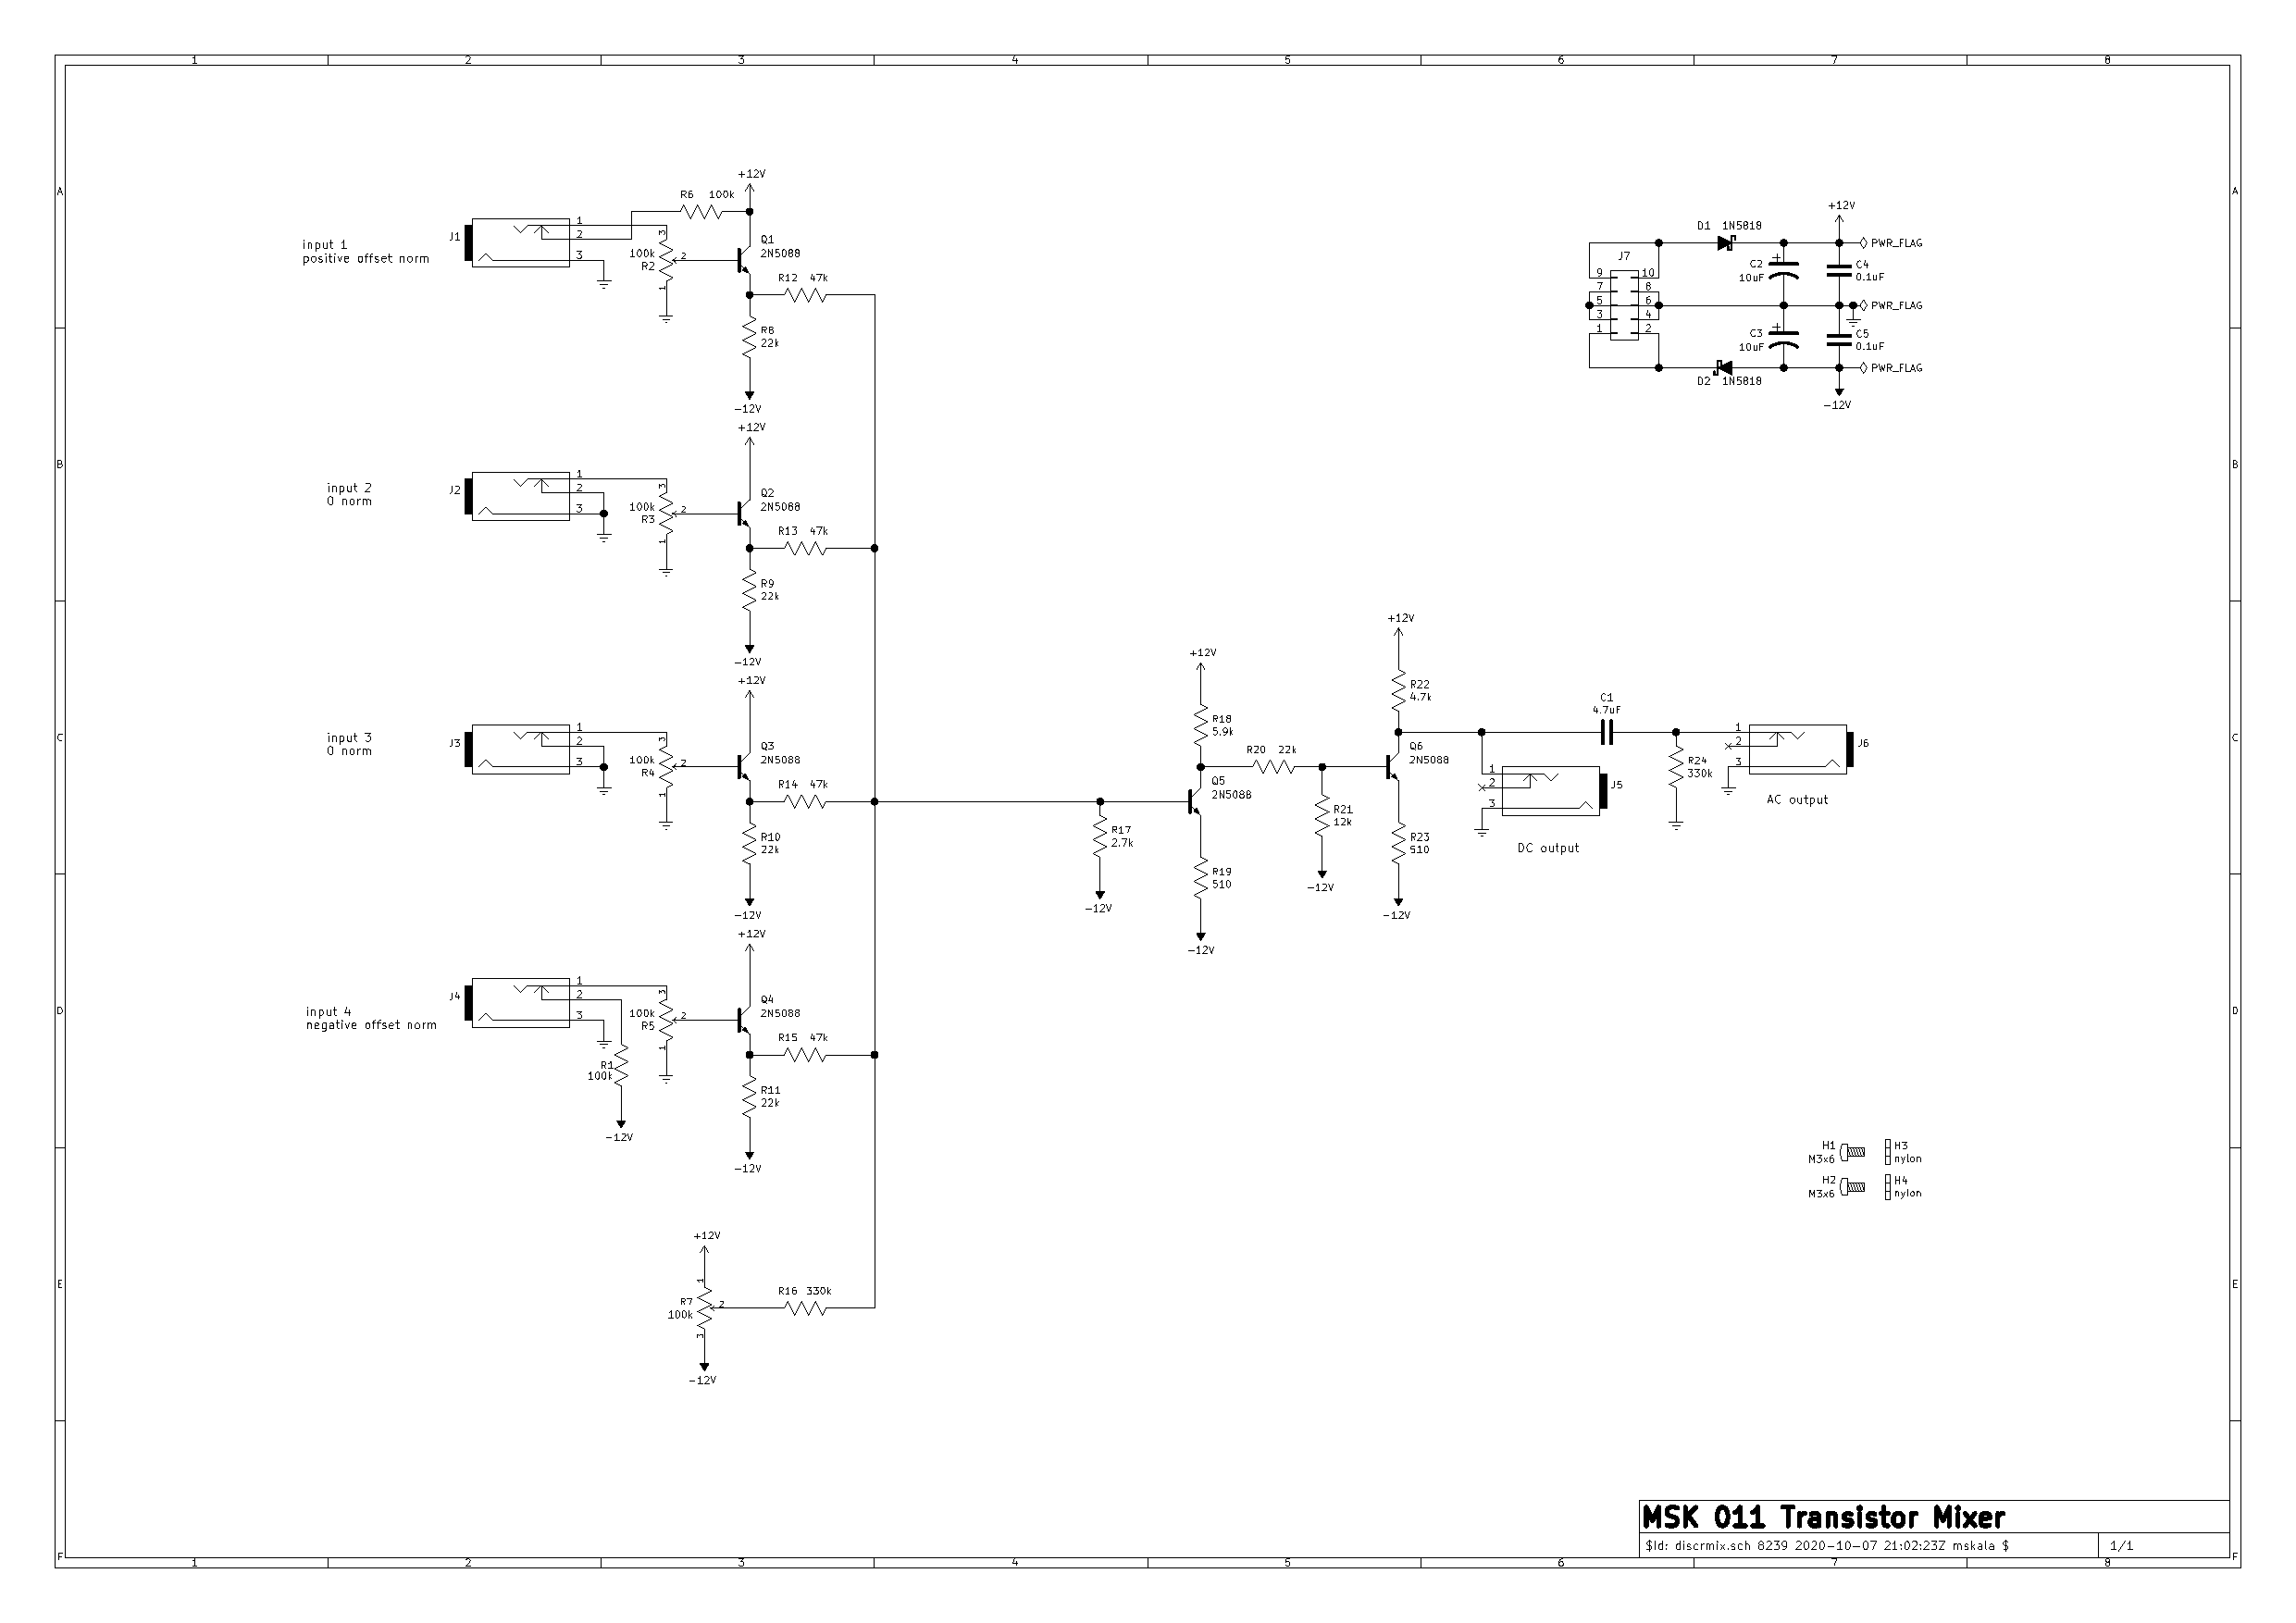
\includepdf[pages=-,angle=90]{schematic.pdf}

\thispagestyle{empty}
\onecolumn
\vspace*{\fill}\begin{center}
\setlength{\fboxsep}{0pt}%
\setlength{\fboxrule}{1pt}%
\fbox{\includegraphics{panel-mockup.pdf}}
\end{center}
\vspace*{\fill}

\clearpage
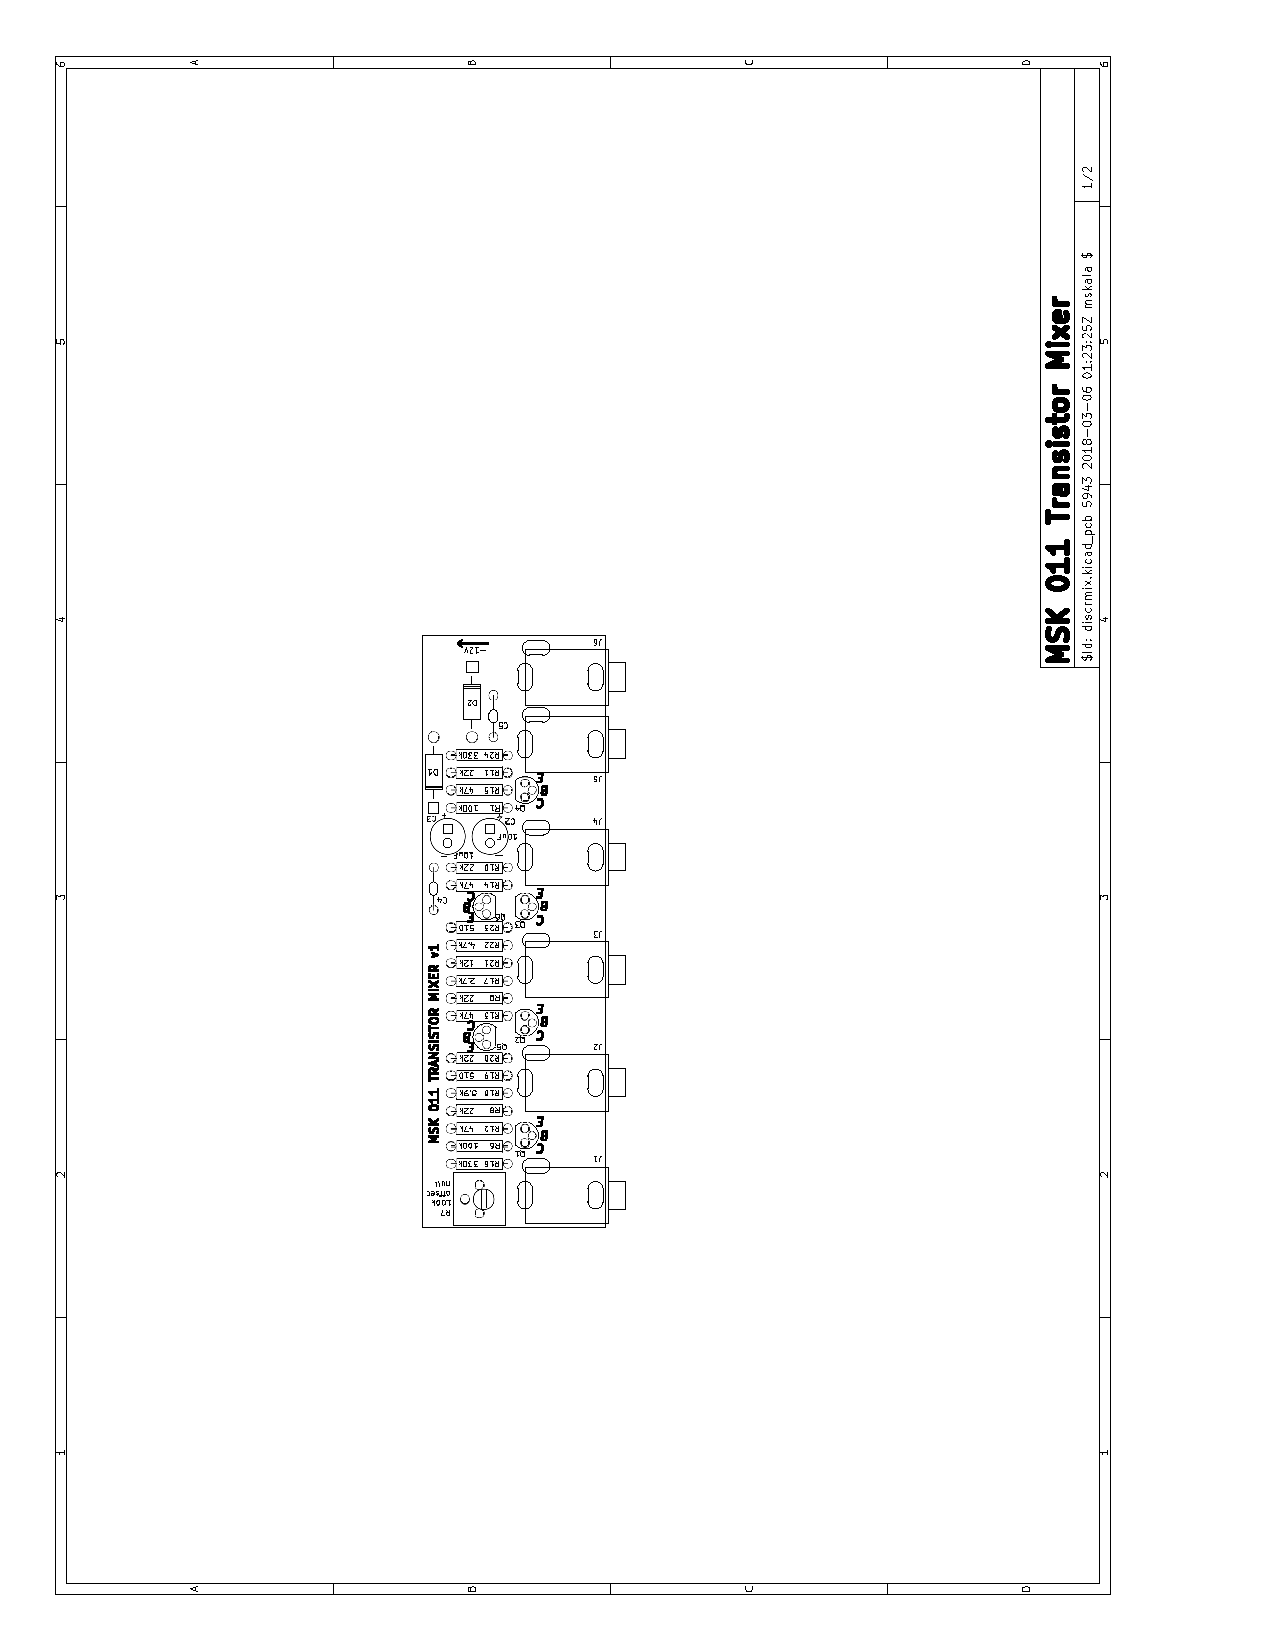
\includepdf[pages=-]{topass.pdf}
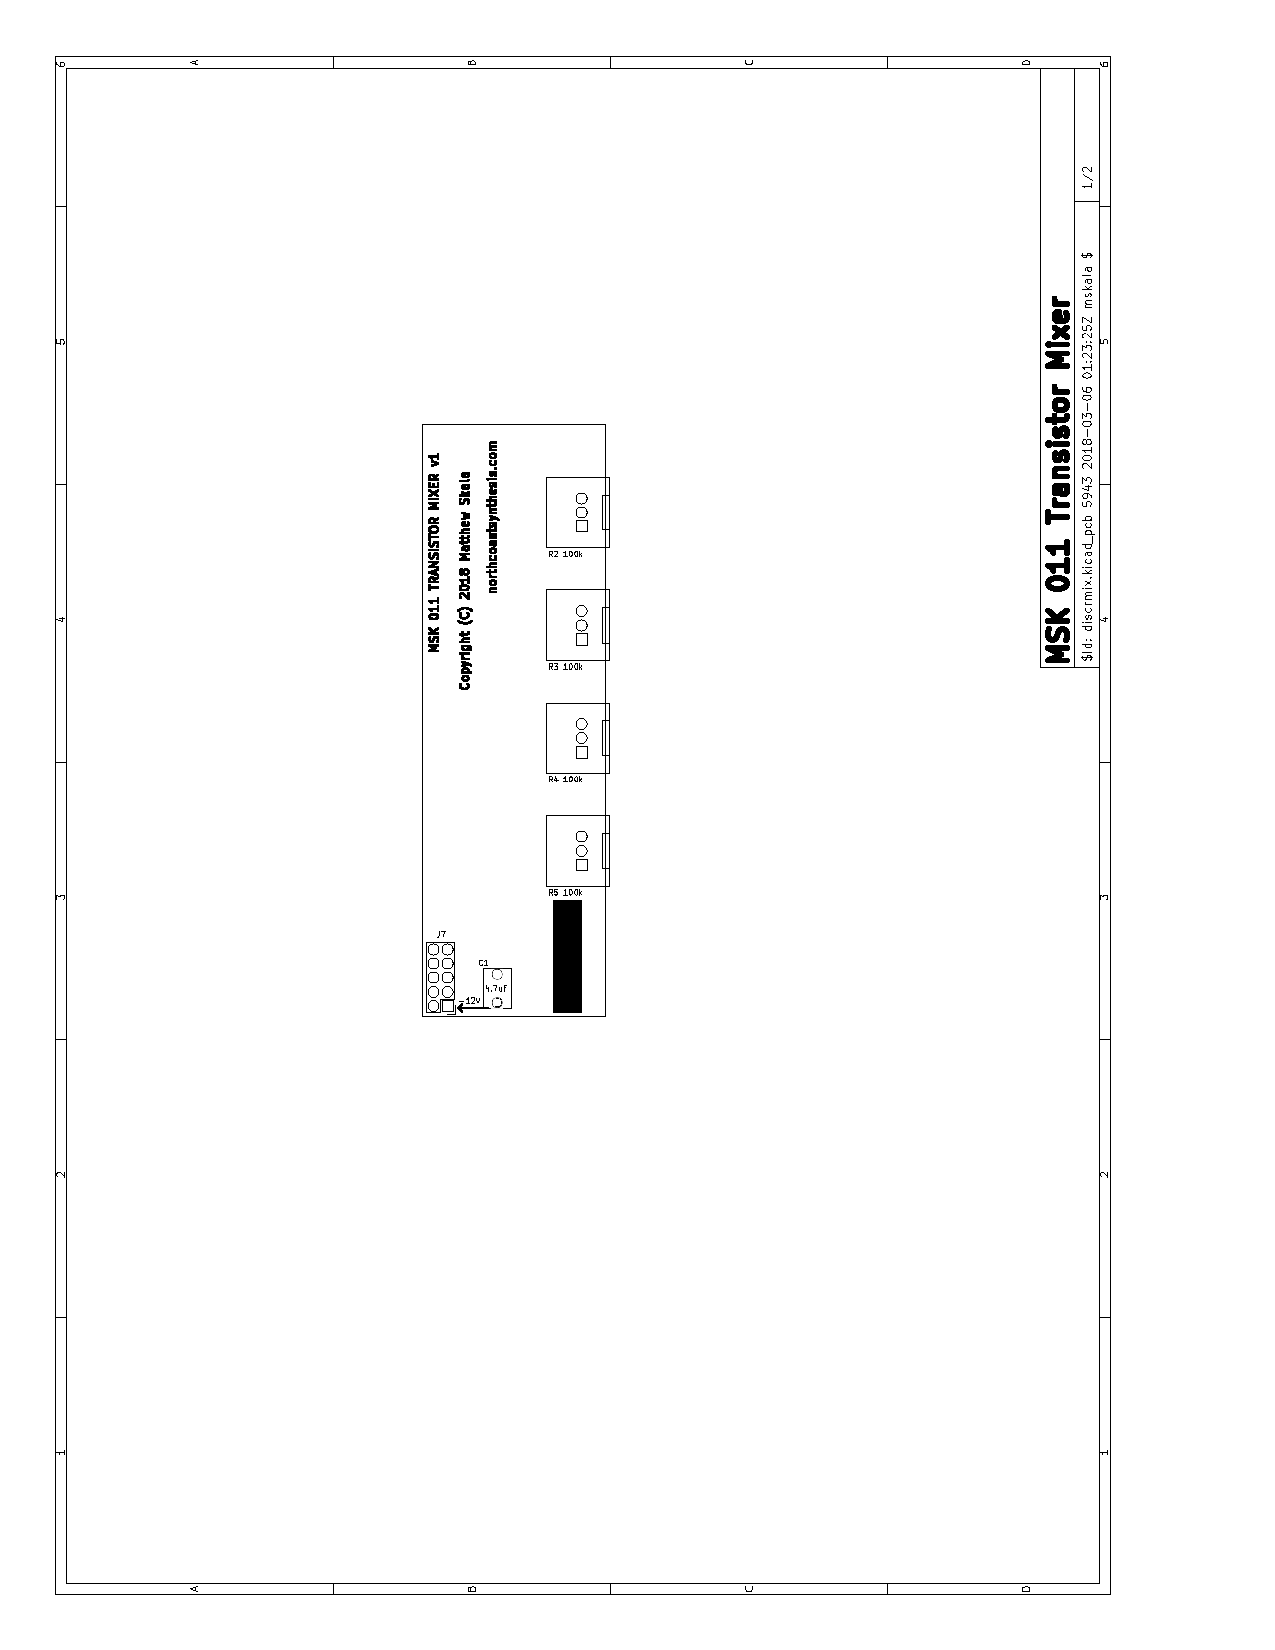
\includepdf[pages=-]{botass.pdf}
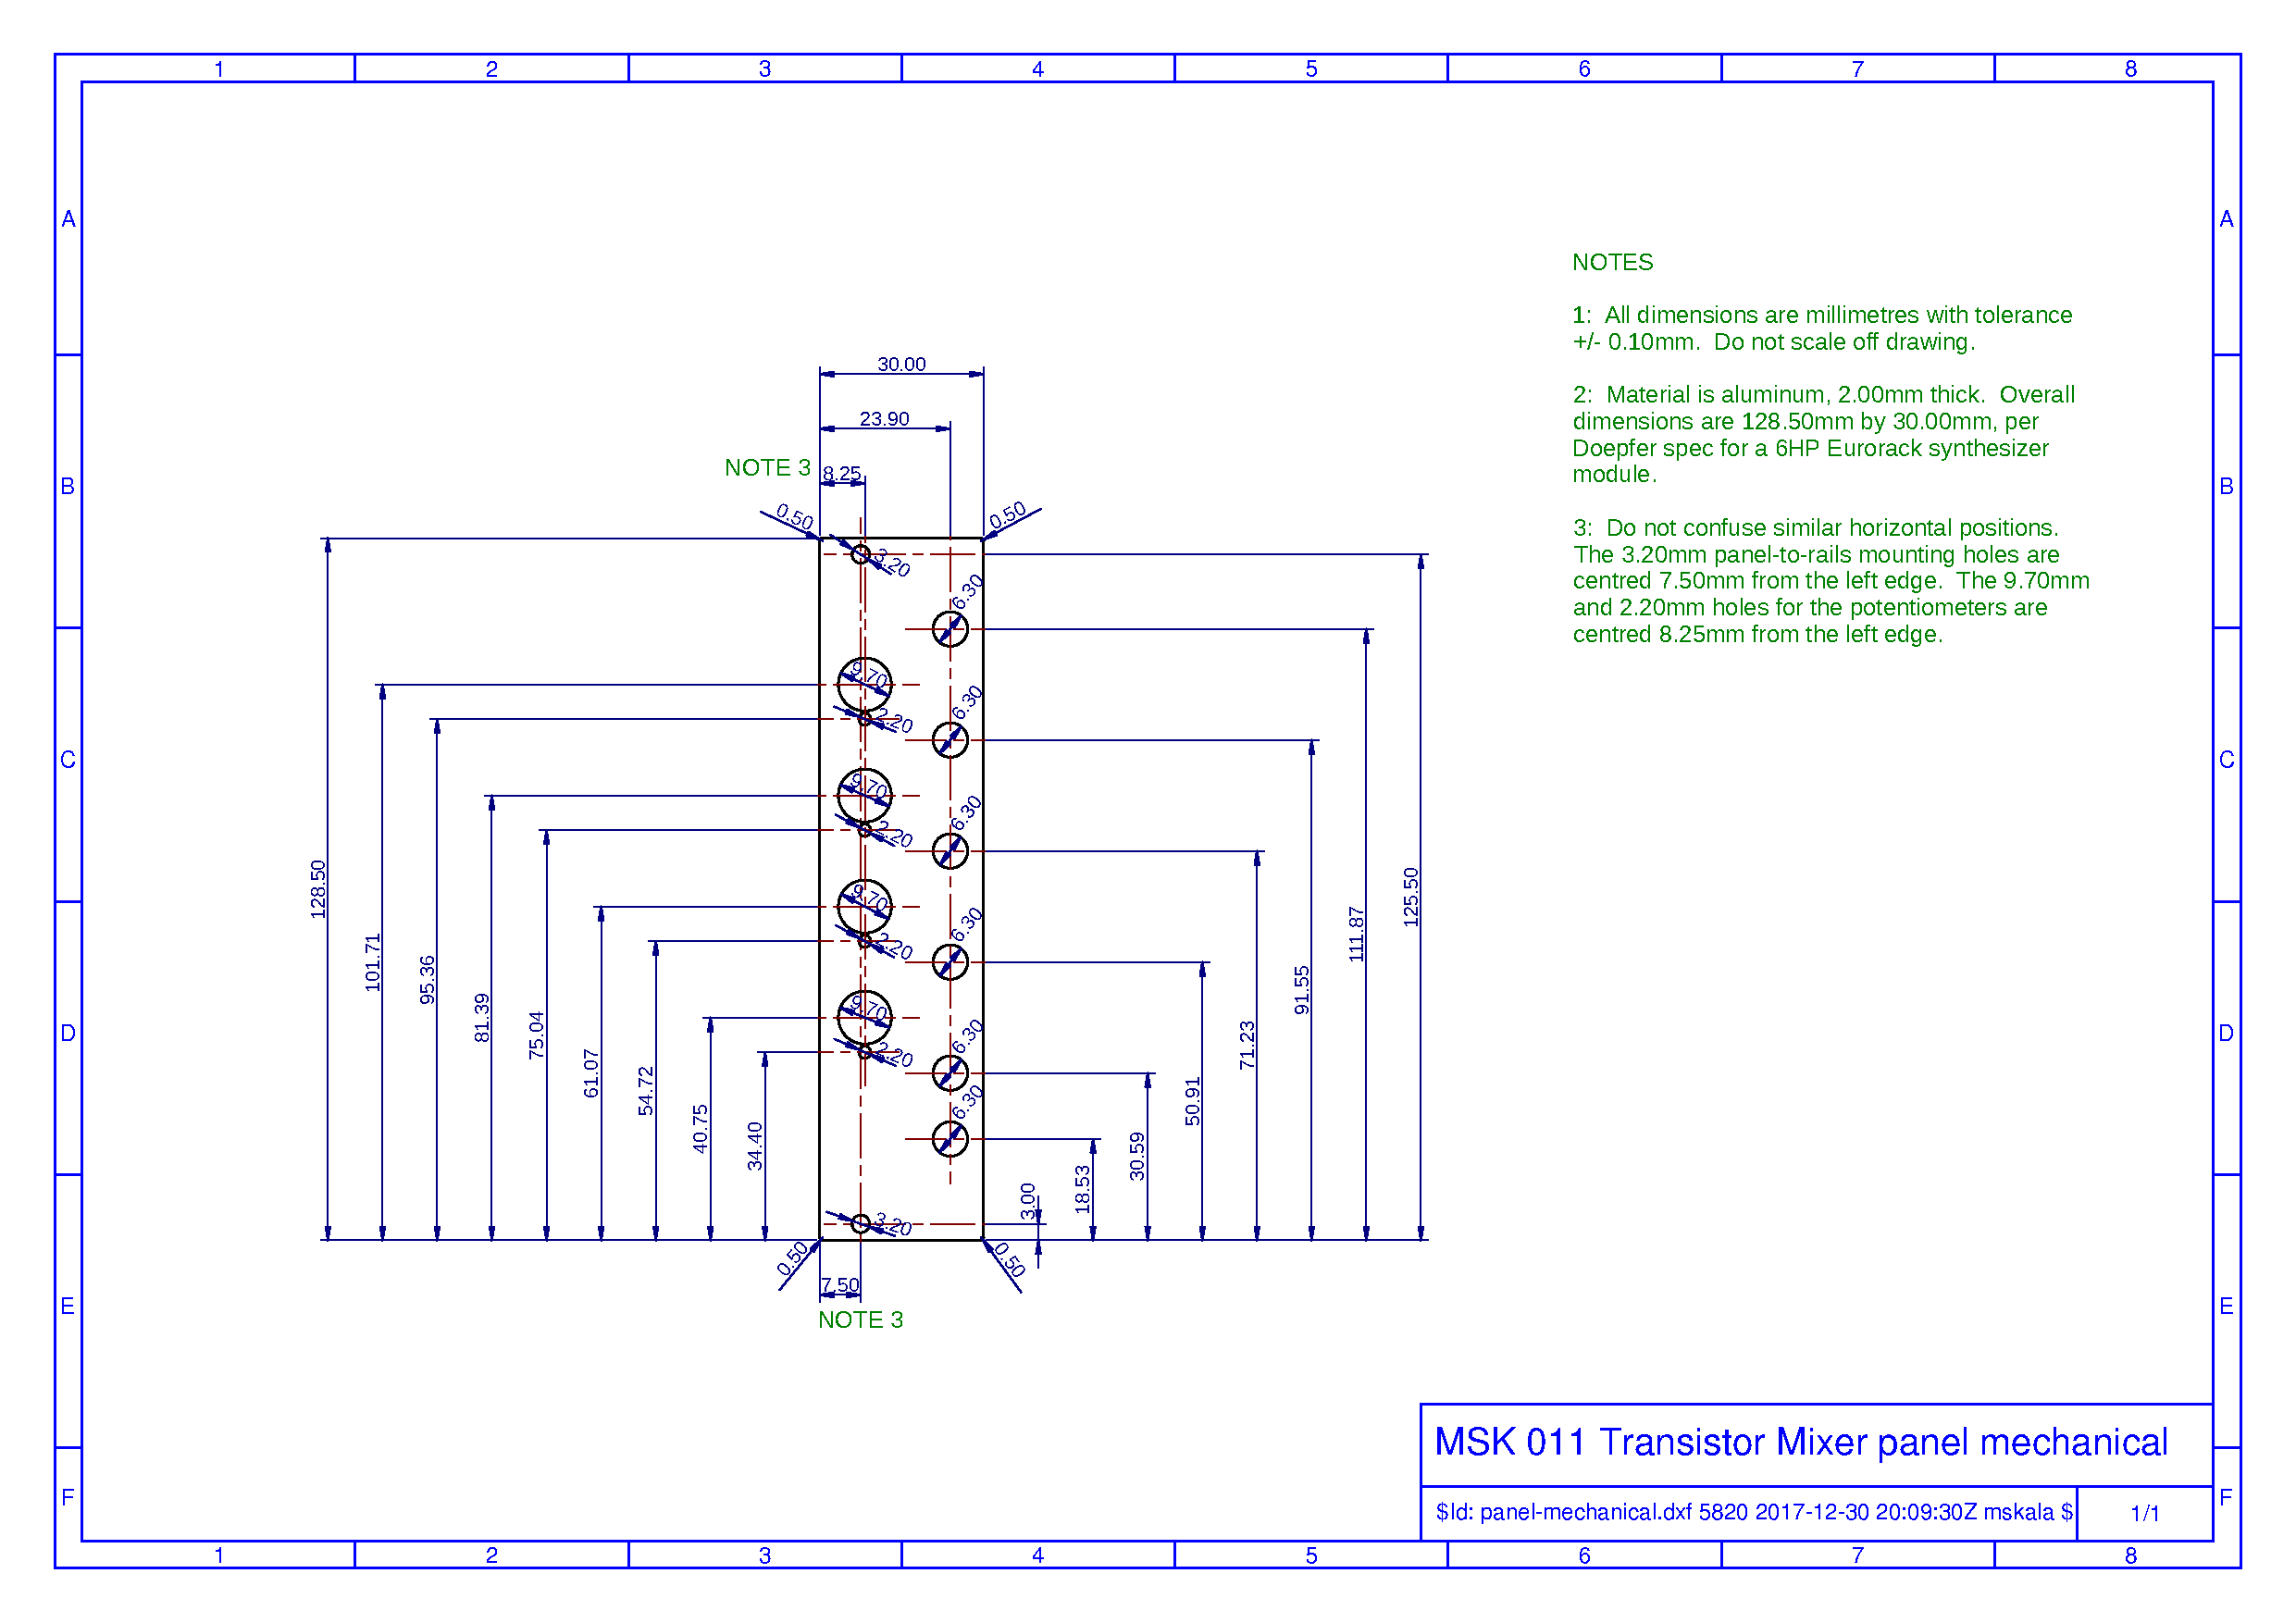
\includepdf[pages=-,angle=90]{panel-mechanical.pdf}
\clearpage\label{fig:exploded}
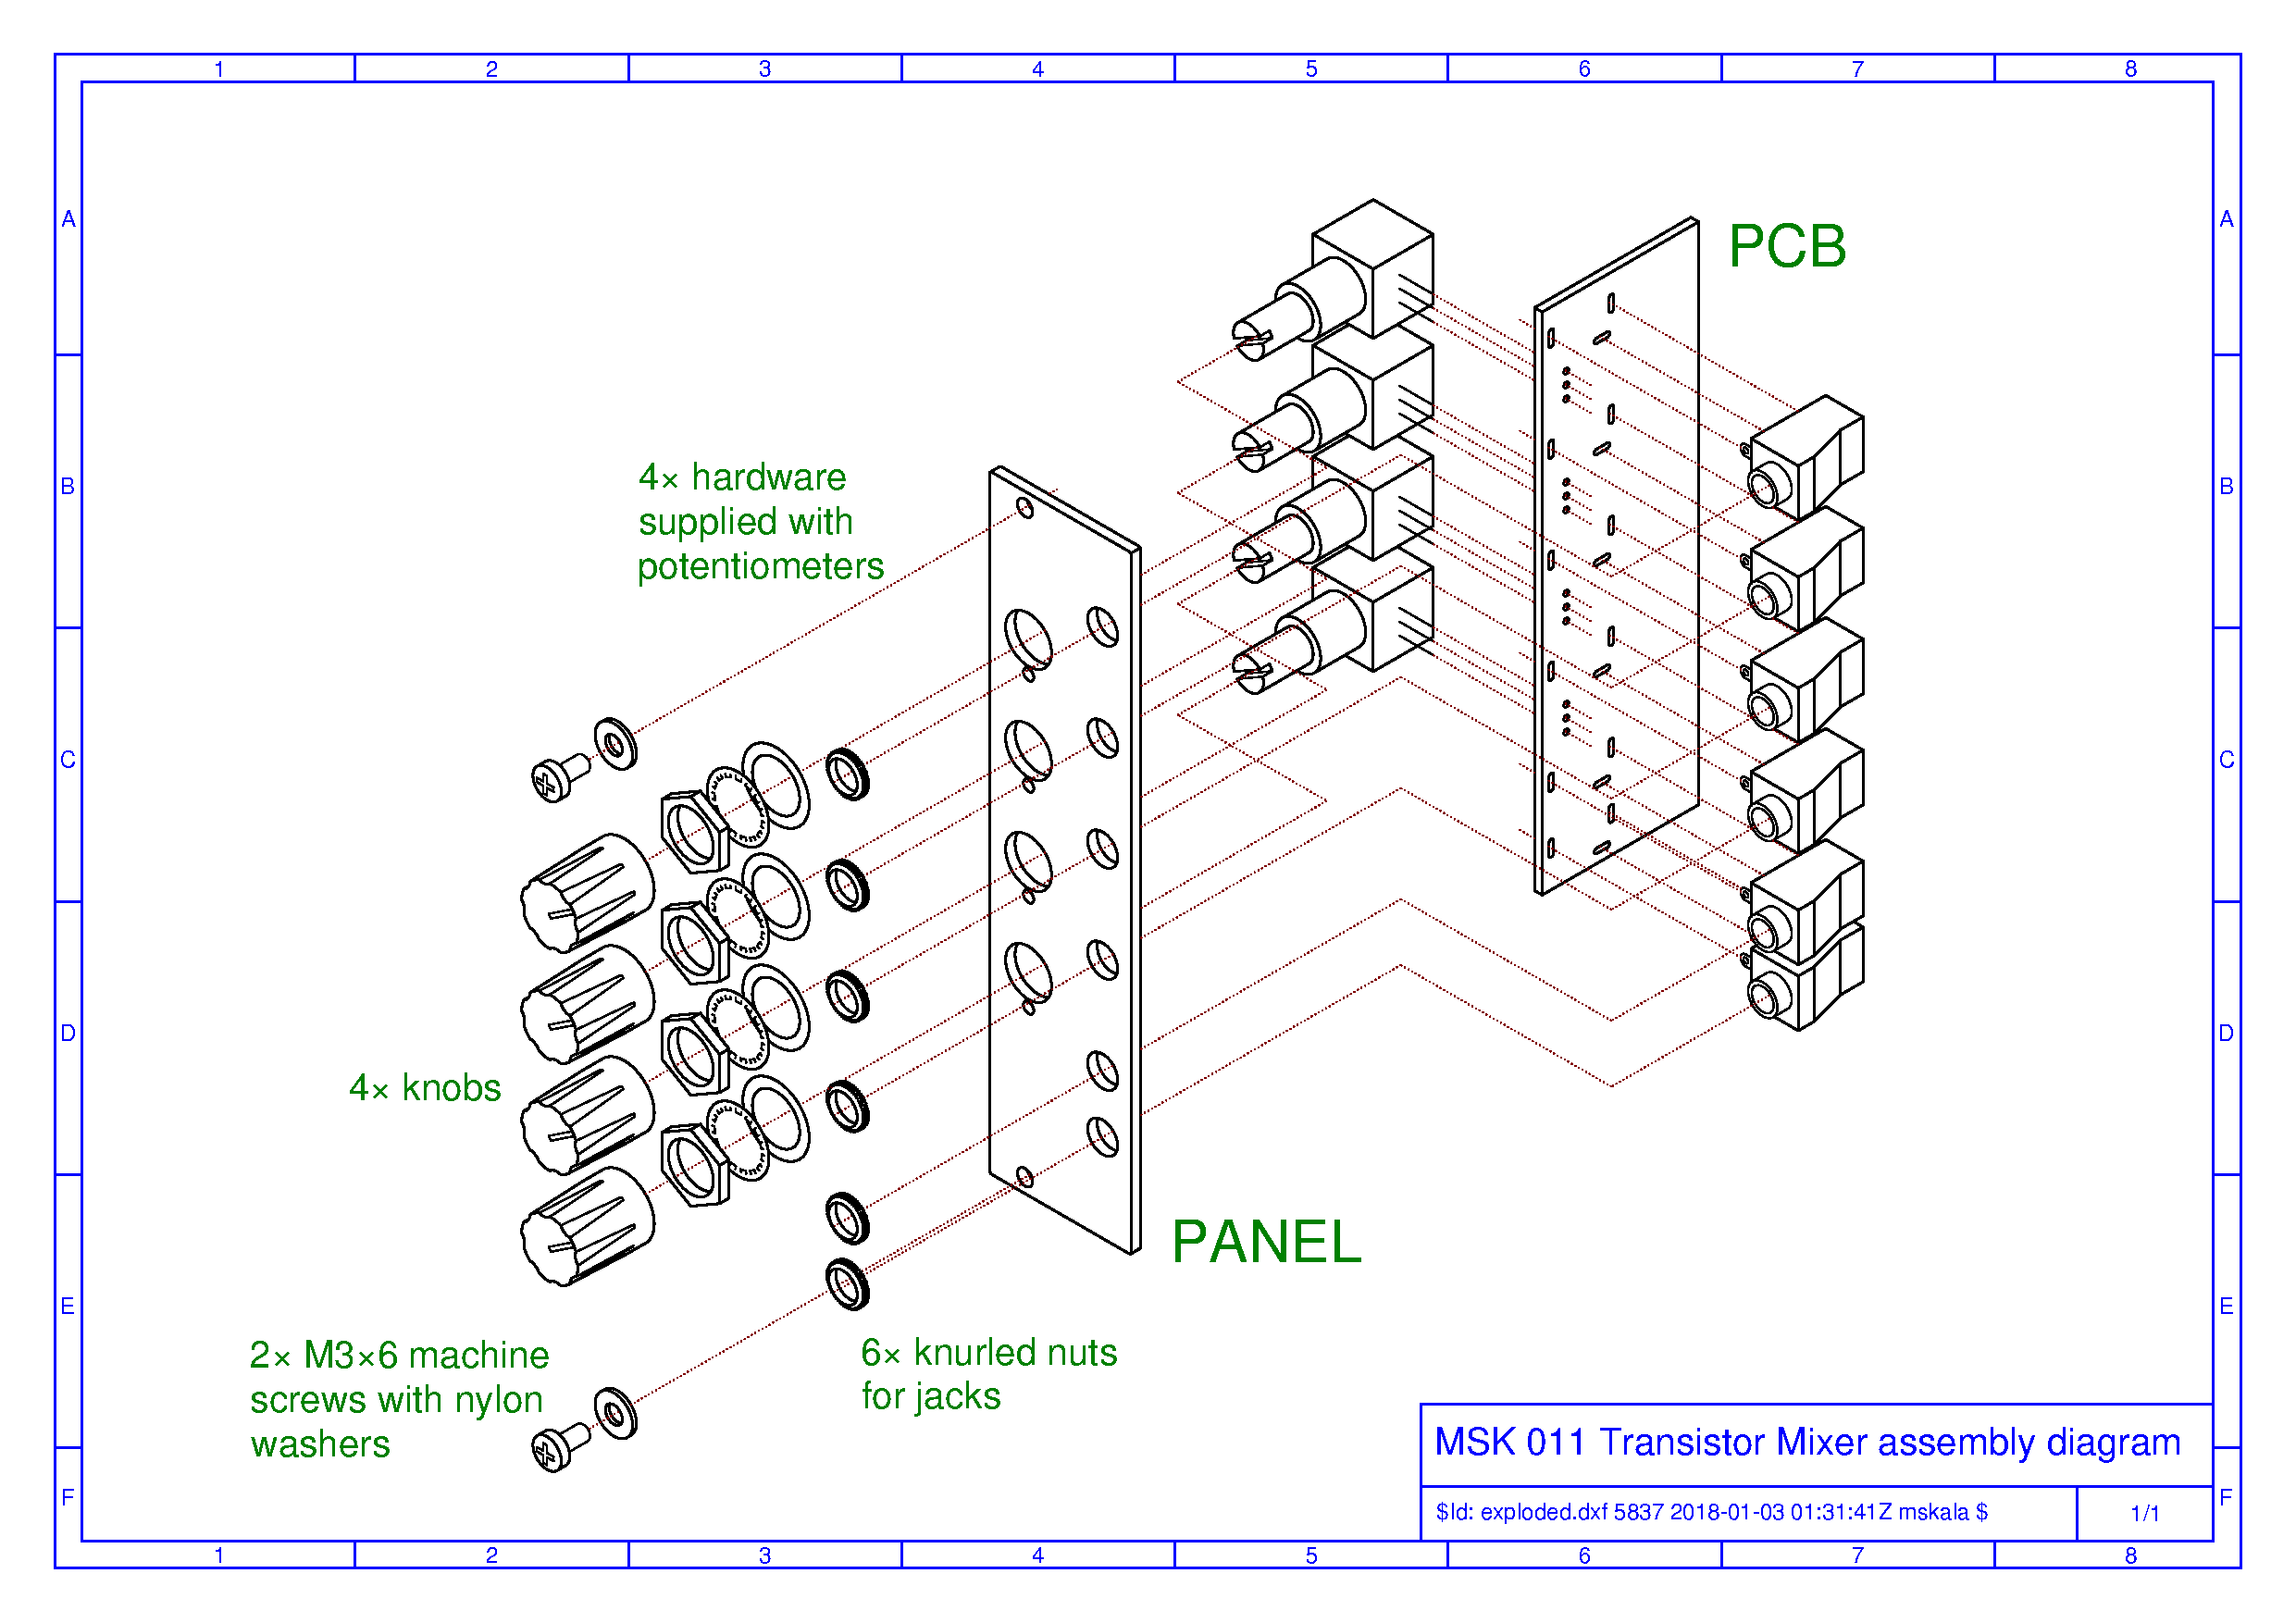
\includepdf[pages=-,angle=90]{exploded.pdf}
